\RequirePackage{amsmath}
\documentclass[runningheads]{llncs}
\usepackage[utf8]{inputenc}
\usepackage{hyperref}
\usepackage{graphicx}
\usepackage{url}

\usepackage{bm}
\usepackage{amssymb}

\usepackage[linesnumbered,ruled,vlined]{algorithm2e}
\SetKwInput{KwInput}{Input}
\SetKwInput{KwOutput}{Output}

\title{Anomaly Detection in Multi-Robot Systems Exploiting Self-Awareness}

\author{Mohammad Rahmani \inst{1}\orcidID{0000-0003-3273-2487} \and Bernhard Rinner \inst{2}\orcidID{0000-0002-8793-3828}}
\authorrunning{M. Rahmani and B. Rinner}
\institute{Digital Age Research Center (DECIDE doctoral school), University of Klagenfurt, Austria. Email: \email{mohammad.rahmani@aau.at} \and Institute of Networked and Embedded Systems, University of Klagenfurt, Austria. Email: \email{bernhard.rinner@aau.at}}

\begin{document}
\maketitle
\begin{abstract}
Self-awareness is intelligent agents' capability to become aware of new experiences using their sensory data. This paper focuses on anomaly detection following principles of self-awareness and proposes coupled hierarchical dynamic Bayesian networks (DBN)  as causal-temporal models to learn cooperative multi-robot behaviors from sensory data. These trained models allow anomaly detection whenever an observed behavior deviates from the learned behavior. We evaluated our approach with a two-drone leader-follower setup where the drones with GPS and LIDAR sensors conduct different maneuvers. Our simulation study shows that coupled DBNs trained with independent sensory data achieve better anomaly detection than DBNs trained with aggregated sensory data. 

\keywords Self-awareness \and anomaly detection \and multi-robot systems \and hierarchical state estimation
\end{abstract}

\section{Introduction}
Self-awareness (SA) is intelligent agents' capability to become the subject of their own attention such that they become aware of new experiences to memorize and retrieve in future use cases \cite{bellman-2020-self-aware-cyber-physical-systems}.  An experience is a causal-temporal phenomenon that establishes a relation between the states' evolution and sensory observations of an agent. A state is an abstraction of the agent and its environment and is important for the representation and execution of tasks by the agent. Causality allows the agents to estimate their state based on the most recent sensory observations. Temporality allows the agents to predict future states based on the current state. 

SA is founded on causal-temporal reasoning in general, and building and using causal-temporal models are essential for SA in a computational context \cite{dutt-2020-self-awareness-for-autonomous-systems}. Learning techniques are mostly used to create appropriate model structures and initialize model parameters. Dedicated SA frameworks have been particularly proposed for robotic systems and comprise modeling and data processing techniques to achieve appropriate SA capabilities \cite{regazzoni-2020-multi-sensorial-generative-and-descriptive-self-awareness-models-for-autonomous-systems}. To create and train causal-temporal models, the robot tries to match the model with the observation, i.e., the robot estimates its state and the state of the environment with its proprioceptive and exteroceptive sensors, respectively, and adapts the model parameters such that the deviation between predicted and observed states remains low. A large deviation indicates an anomaly between model and observation and may trigger the creation of a new model which better matches the recent observations. 
    
This paper focuses on anomaly detection following principles of self-awareness. We propose a hierarchical causal-temporal modeling for multiple robots that cooperatively achieve specific missions. Hierarchical modeling supports different abstractions of the robot's state space and improves decision making.  We initialize these models by observing scenarios and use them to detect anomalies. Figure~\ref{fig-framework} depicts our proposed approach where proprioceptive and exteroceptive sensor data is preprocessed and either forwarded to offline learning or online anomaly detection. In offline learning, coupled hierarchical dynamic Bayesian network (DBN) models are separately learned from the observed internal (proprioceptive) state of the robots and the (exteroceptive) state of the environment. In online testing, predicted states are compared with the current observation in order to detect anomalies that may trigger updating existing models or creating new ones.

The contribution of this paper includes (i) the adaption of a SA framework for hierarchical modeling and anomaly detection in multi-robot systems \cite{regazzoni-2020-multi-sensorial-generative-and-descriptive-self-awareness-models-for-autonomous-systems}, (ii) an analysis of parameters that effects anomaly signals, and (iii) a simulation study using different multi-robot scenarios with GPS and LIDAR sensors. 
Similar to \cite{baydoun-2018-learning-switching-models-for-abnormality-detection-for-autonomous-driving,baydoun-2019-prediction-of-multi-target-dynamics-using-discrete-descriptors-an-interactive-approach} our work is founded on hierarchical DBNs for causal-temporal modeling and anomaly detection. However, our work distinguishes proprioceptive and exteroceptive models, applies different clustering techniques and anomaly metrics, and reduces the dimensionality of exteroceptive sensory data with autoencoders \cite{wang-2016-auto-encoder-based-dimensionality-reduction}. A preliminary version is sketched in \cite{rahmani-2022-towards-self-awareness-in-multi-robot-systems}. 

\begin{figure}
  \centering
  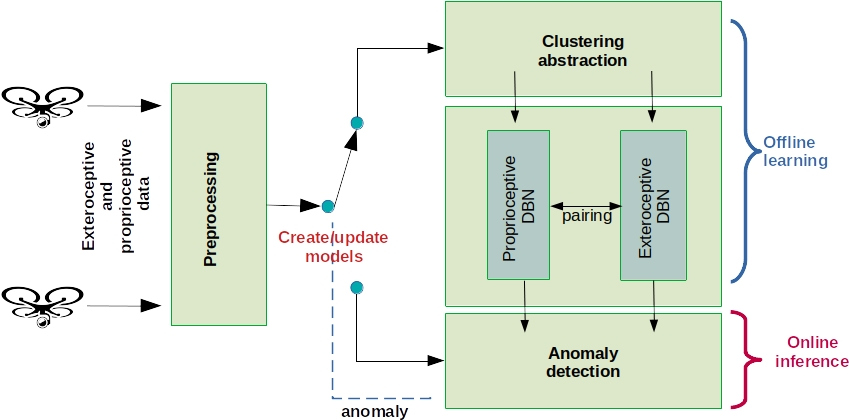
\includegraphics[width=0.8\textwidth]{assets/framework.jpg}
  \caption{The proposed SA framework learns offline proprioceptive and exteroceptive models which are used for online anomaly detection. A detected anomaly may trigger updating existing models or creating new models.}
  \label{fig-framework}
\end{figure}

The remainder of this paper is organized as follows: Section~\ref{sec-related-work} discusses related work. Section~\ref{sec-single-dbn} introduces hierarchical DBNs as a causal-temporal model for a single robot. Section~\ref{sec-coupled-dbn} expands DBN-based models to multiple robots and presents details of anomaly detection. Section~\ref{sec-results} discusses the results of our simulation study. Finally, Section~\ref{sec-conclusion} concludes the paper.
 
\section{Related Work}
\label{sec-related-work}

Related work in SA frameworks can be grouped into two categories: (i) biologically-inspired theories about causal-temporal models and the processing of proprioceptive and exteroceptive sensory data and (ii) computational implementations of these theories. 
Damasio \cite{damasio-2003-looking-for-spinoza-joy-sorrow-and-the-feeling-brain}, Haykin \cite{haykin-2012-cognitive-dynamic-systems-perception-action-cycle-radar-and-radio}, and Friston \cite{friston-2014-cognitive-dynamics-from-attractors-to-active-inference} introduced three bio-inspired SA modeling theories. We refer to \cite{regazzoni-2020-multi-sensorial-generative-and-descriptive-self-awareness-models-for-autonomous-systems} for a detailed discussion of these theories. 

From the computational implementation perspective two main approaches are worth mentioning. The first approach exploits deep learning techniques. For example, Long Short-Term Memory (LSTM) \cite{hochreiter-1997-long-short-term-memory} networks can be used as temporal models for sequential data predictions and forecasting time series. However, traditional deep learning approaches face limitations in causal modelling and they represent black boxes which require many model parameters and a huge training set. They can further hardly provide any certainty rate over their predictions.

The second approach is founded on DBNs which are data-driven Probabilistic Graphical Models (PGM) \cite{koller-2009-probabilistic-graphical-models-principles-and-techniques}  that can be used as causal-temporal models. They use Bayesian filtering methods at different levels of their hierarchy to predict and estimate the current state and to detect anomalies according to the most recent sensory observations. They build temporal relations between the states according to the data derived during initialization and consequently, in a new experience, they update the posterior probability of the agent's state space based on this observation. 

Switching Dynamical Linear System (SDLS) \cite{sudderth-2009-nonparametric-bayesian-learning-of-switching-linear-dynamical-systems} are special hierarchical DBNs that can represent a dynamic non-linear system as a set of linear models. They use discrete random switching variables associated with these linear dynamic models at higher levels of the DBN to recursively estimate the joint posterior of the state and the switching variables.   
Markov Jump Particle Filter (MJPF) \cite{baydoun-2018-learning-switching-models-for-abnormality-detection-for-autonomous-driving}  is one such switching model that uses a two-time slice DBN \cite{koller-2001-sampling-in-factored-dynamic-systems} for causal-temporal reasoning at lower continuous and higher discrete levels. At the continuous level, it uses a bank of Kalman Filters (KF) which are associated with linear dynamic models derived from abstract states. These abstract states correspond to particles of a Particle Filter (PF) at the discrete level from which the aforementioned KFs get the control vector of the dynamic system to predict the next continuous state. MJPF has been used in a variety of dynamic systems. For example, Kanapram et al.~\cite{kanapram-2021-dynamic-bayesian-collective-awareness-models-for-a-network-of-ego-things} have used it for anomaly detection and implementing collective awareness in connected autonomous vehicles. 

None of these approaches offer a solution toward SA in MRS to cooperatively accomplishing a task. However, \cite{kanapram-2021-dynamic-bayesian-collective-awareness-models-for-a-network-of-ego-things,baydoun-2019-prediction-of-multi-target-dynamics-using-discrete-descriptors-an-interactive-approach} are the closest related works to our approach. The first one applies a distributed set of causal-temporal models to detect an anomaly in the behavior of other robots. The second one uses coupled causal-temporal models to learn the behavior of an involving robot in a mission by another robot.   

\section{Hierarchical DBN Modeling}
\label{sec-single-dbn}
We adopt DBNs for our modeling approach by clustering the sequence of observed sensory data $Z$ obtained during accomplishing a task into a set of quasi-stationary regions. A hierarchical modeling is achieved by representing the behavior within a region by a (continuous) state $X$ and each region by an abstracted state $S$. We represent the state $X$ of the robot as a generalized state up to the first derivative leading to the following state formulation
    \begin{equation}
        \small
        X = \{\bm{x} \in \mathbb{R}^{2n} | \bm{x}=[x_1,\dots,x_n,\dot{x}_1,\dots,\dot{x}_n]^T \}
        \label{eq-state-space-morphology}
    \end{equation} 
    where $\dot{x}_i$ is the first derivative of $x_i$ and $n$ represents the state dimension. 
    
The relation between sensory observations and states is established by an observation model $Z_t = H\bm{x}_t + \nu_t$ where $\bm{x}_t$ is a given state at time $t$, $H$ is the observation matrix and $\nu_t$ is the observation, zero-mean, Gaussian noise vector with the covariance $R$, i.e., $\nu_k \sim \mathcal{N}(0,R)$.  
In this work we assume that the state has the same morphology as the observation. Thus, $H$ is the identity matrix $I_{2n}$. $z = \{\bm{z}_0,\dots,\bm{z}_m\}$ represents the raw observation data from the robot during $m+1$ time steps. In the \textit{preprocessing} step, data normalization is performed and derivatives are included to the observation
\begin{equation}
    \small
     Z = \{Z_t=[\alpha I_n \bm{z}_t,\beta I_n \frac{\bm{z}_t-\bm{z}_{t-1}}{\Delta t}]^T | t \in \{1,\ldots,m\}\}
\end{equation}
with $\Delta t$ as sampling time.
$\alpha$ and $\beta$ are real numbers such that $\beta>\alpha$ and $\alpha+\beta=1$ for weighting the raw observations and first derivatives, respectively. This helps to improve the succeeding data clustering such that the clustering mechanism favors patterns with smaller variations of the derivatives to cluster quasi-stationary regions.

\subsection{Offline Training}
\label{sec-single-robot-offline-training}
The offline phase begins with clustering weighted observations. In the \textit{clustering} step, we partition the weighted observations into $p$ clusters 
    \begin{equation}
        \small
        S=\{S_1,\dots,S_{p}\}.
        \label{eq-abstract-states}
    \end{equation}
$\mu_i$ and $\Sigma_i$ represent the mean and covariance of cluster $S_i$. A quasi-stationary region is defined as a neighborhood  
    \begin{equation}
        \small
        N_i = N_{\mu_i}(3\sqrt{tr(\Sigma_i)})
    \end{equation}
where the mean $\mu_i$ is its center and $3\sqrt{tr(\Sigma_i)}$ is its radius with $tr(.)$ as the trace operator. Areas outside of any neighborhood are referred as unknown regions.

The following process model can thus be specified for each region
    \begin{equation}
        \small
        X_{t} = FX_{t-1}+BU_{S_{t-1}}+\omega_{t-1}
        \label{eq-process-model}
    \end{equation}
    where 
    \begin{equation}
        \small
        F = 
        \begin{pmatrix}
        I_n & 0_n \\
        0_n & 0_n 
        \end{pmatrix}
    \end{equation}
    represents a transition matrix. 
    $B = [I_n \Delta t \ I_n]^T $ is the control matrix, and $U_{S_{t-1}}=[I_n \ 0_n]\mu_{S_{t-1}}$ is the control vector. The process noise $\omega_{t-1}$ is drawn from a zero-mean, Gaussian distribution such that $\omega_{t-1} \sim \mathcal{N}(0,\Sigma_{S_{t-1}})$.

   Now, we can formalize the hierarchical, causal-temporal model (cp.~the colored boxes in Figure~\ref{fig-cdbn}) for initialization. The single robot model is composed by observations $Z$, continuous states $X$ and abstract states $S$ at individual time points, the transition probabilities $\pi$ between continuous states and between abstract states as well as the occurrence likelihood $\lambda$ between the different levels. In order to initialize the causal-temporal model, observations from the execution of a reference task are used for determining the transition probabilities and the occurrence likelihood during offline training.
    
    For an abstract state $S_i$, we use a KF for representing the state evolution within the region $N_i$ which determines a probability distribution over the continuous state space given the most likely previous continuous state. In other words, we have
    \begin{equation}
        \small
        \pi_{XX} = \{p(\bm{x}_t|\bm{x}_{t-1}, S_{i} | \bm{x}_t \in X)\}
        \label{eq_process-model2}
    \end{equation}
    as probability distribution over $X$ in $N_i$.

We use a PF to determine the posterior of the regions as the transition from one abstract state to the other is not linear. We need a transition matrix among the abstract states. Algorithm~\ref{alg-one-alphabet-transition-matrix} sketches the computation of this transition matrix which represents the following probability distribution
    \begin{equation}
      \small
      \pi_{SS} = \{p(S_{i} \ | \ S_{j})=T_{i,j} \ | \ i,j \in \{1,\dots,p\}\}.
      \label{eq-abstractstate-transition-matrix}
    \end{equation}
This algorithm determines the closest region for the previous and current observation based on the Euclidean distance $d$ (lines 3 and 4). Thus, $i$ and $j$ indicate the corresponding abstract states, and the most probable abstract state $S_{i|j}$ can be derived from the previous abstract state and $\pi_{SS}$.
    \begin{algorithm}
        \caption{Transition matrix for abstract states}
        \label{alg-one-alphabet-transition-matrix}
        \DontPrintSemicolon
        \KwInput{Z}
        \KwOutput{$T_{p \times p}$}
        $T_{p \times p} \gets 0_p$\;
        \For{$t=1$ \KwTo $m$}
        {   
            $i \gets \arg \min_{k=1}^{p} d(Z_{t-1},\mu_k)$\;
            $j \gets \arg \min_{k=1}^{p} d(Z_{t},\mu_k)$\;
            $T_{ij} \gets T_{ij}+\frac{1}{m}$\;
        }
    \end{algorithm}
 We normalize the distances between the center of $S_j$ ($\mu_{j}$) and all observations to [0,1] and compute the occurrence likelihood as
    \begin{equation}
        \small
        \lambda_{XS}=\{p(\bm{x}|S_{i|j}) | \bm{x} \in X\}.
    \end{equation}
    
\begin{figure}[t]
\centering
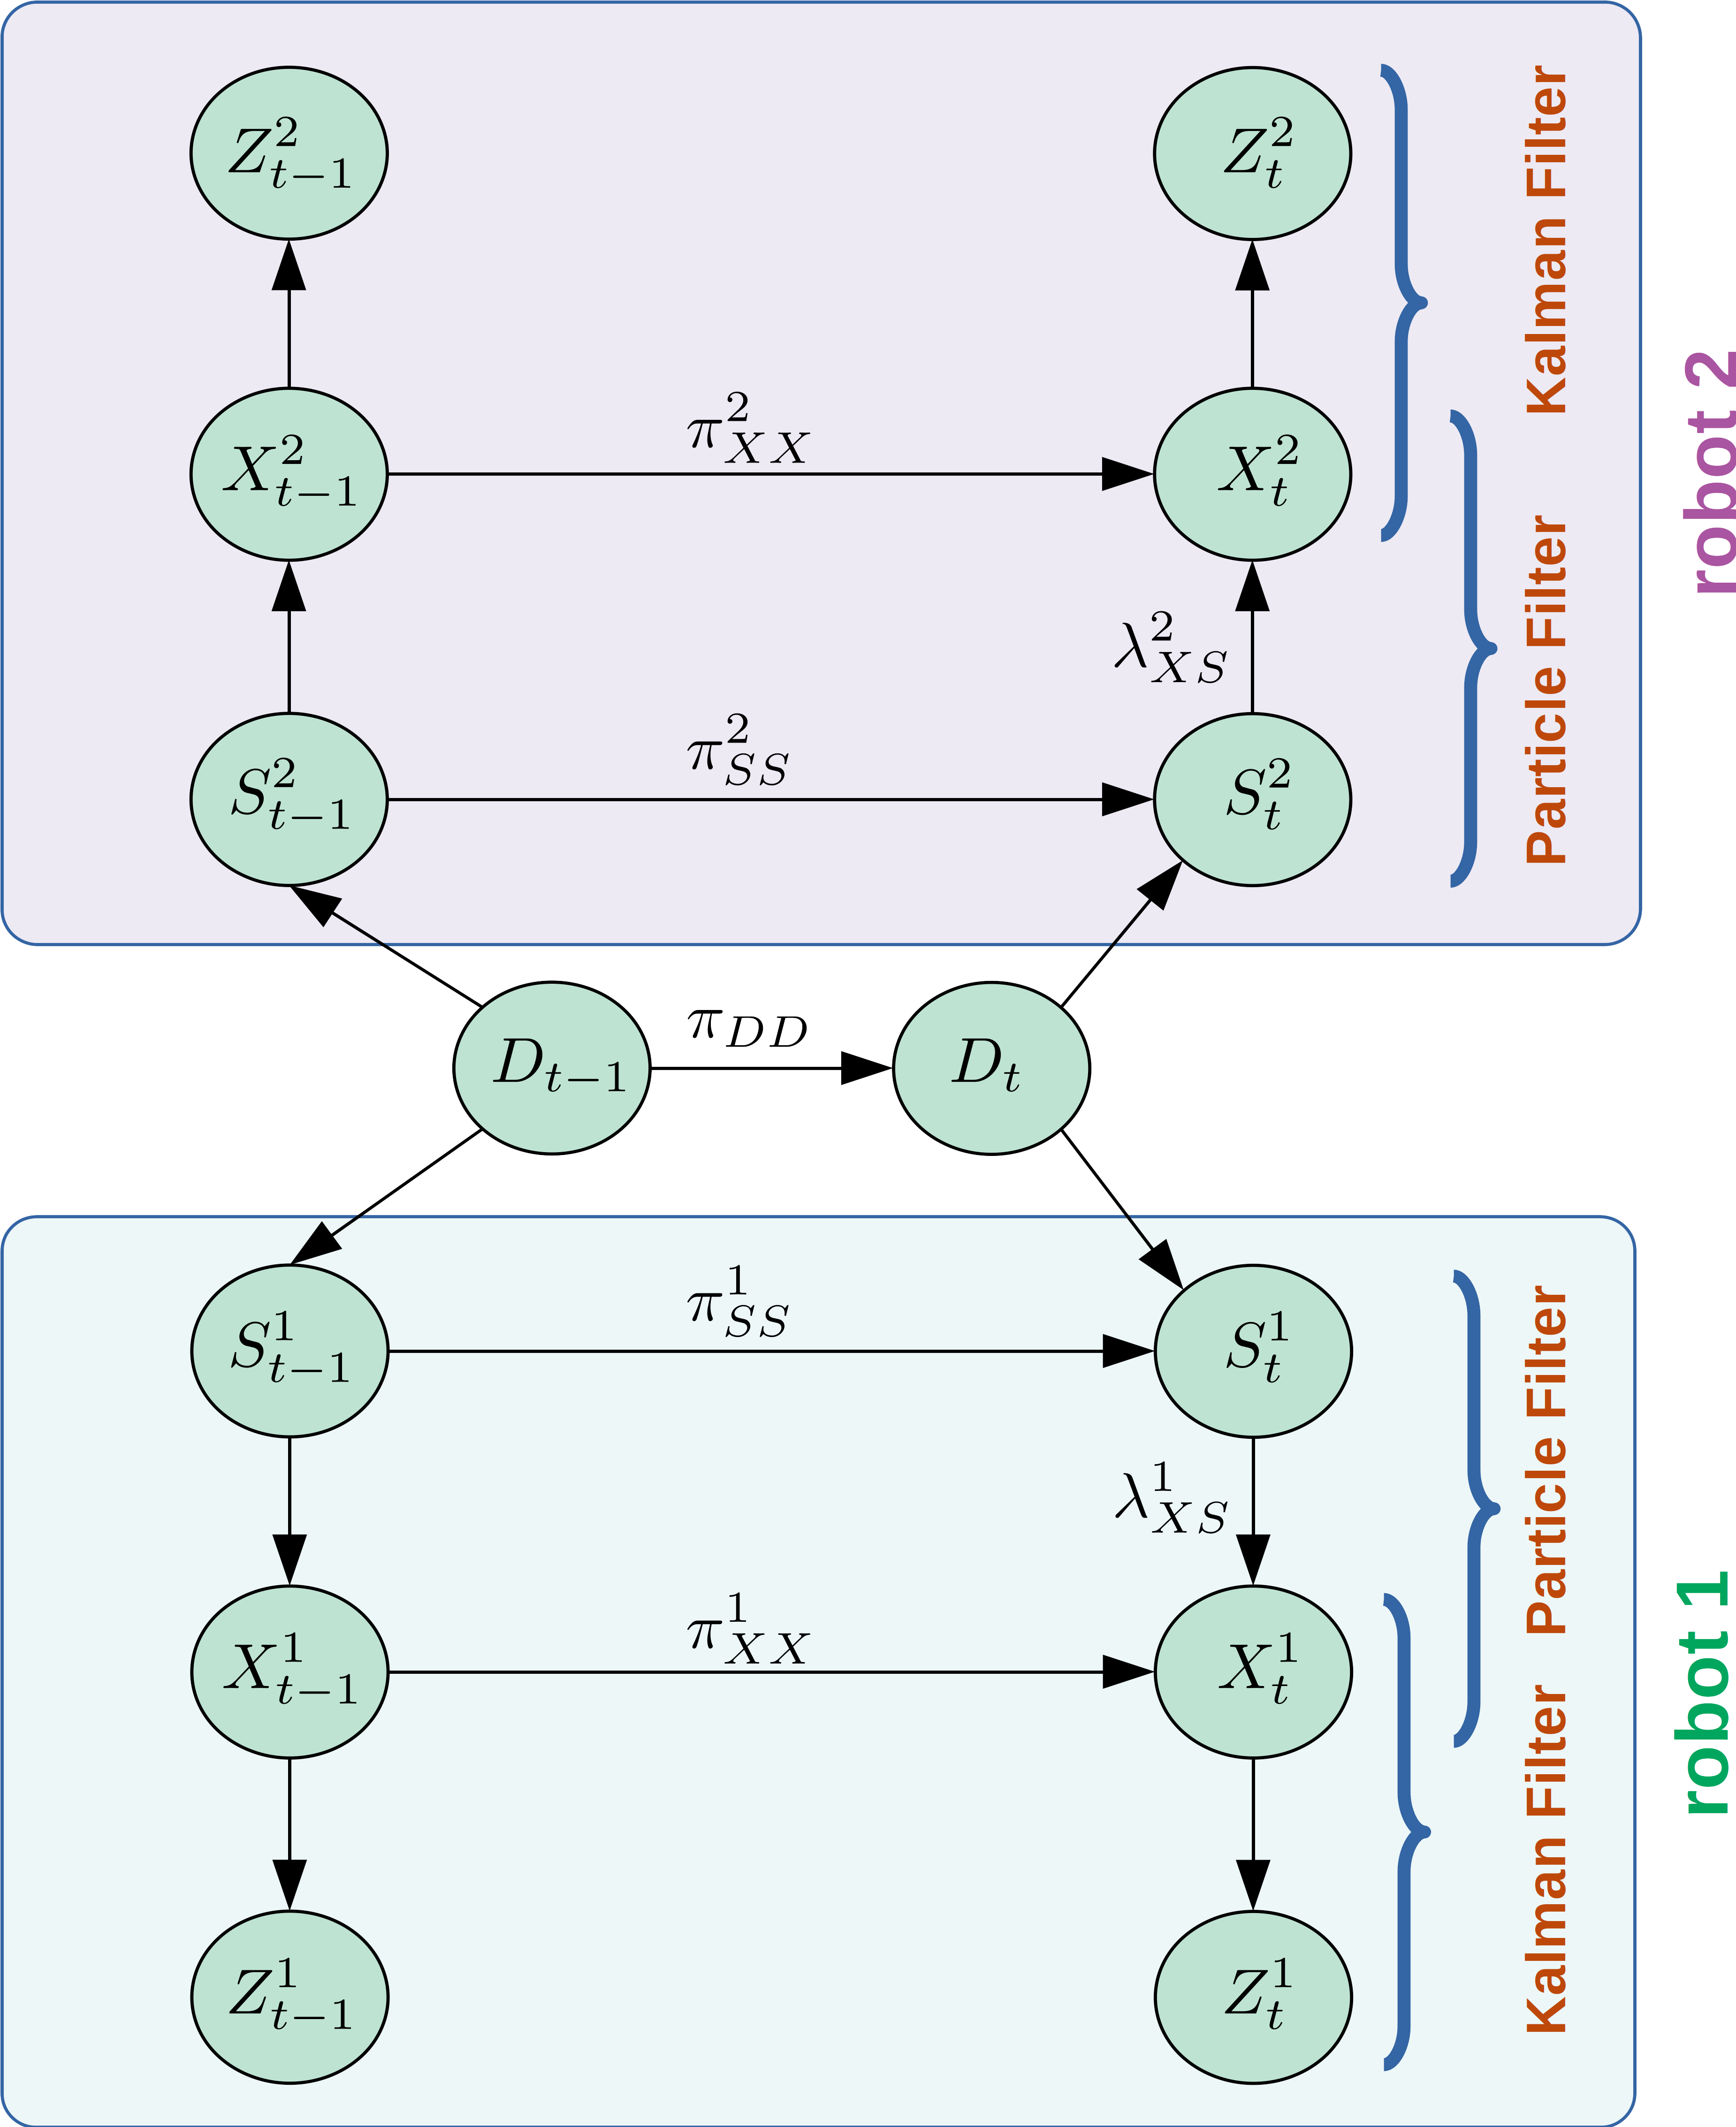
\includegraphics[scale=0.05]{assets/cdbn.png}
\caption{Hierarchical coupled DBN. Horizontal arrows present temporal relationship between random variables at two consequent time steps $t$ and $t-1$. Vertical arrows present the causal relationship between them. $Z$ represents the observation, $X$ the continuous state, $S$ the abstract level state, and $D$ the coupled state. $\pi$ represents the transition probabilities at different levels and $\lambda$ the occurrence likelihood of states according to lower level parameters.}
\label{fig-cdbn}
\end{figure}
       
\subsection{Online Testing}
\label{sec-single-robot-online-testing}

Having $\pi_{SS}$, $\pi_{XX}$ and $\lambda_{XS}$ introduced, we propose a state estimation method based on hierarchical DBNs (cp.~Figure~\ref{fig-cdbn} for individual robots). It uses a PF which is coupled with a bank of KFs at the abstract state level (a dedicated KF for each region) and the continuous state level jointly for state estimation. At the continuous level, states are inferred from observations and  $\pi_{XX}$ predictions are computed by the KF associated with each region. At the abstract level, $\pi_{SS}$ is used by the PF for state estimations. These two levels are related to each other by using the particles in the regions to choose the appropriate KF.
    
The PF uses a set of weighted vectors in the state space to estimate the posterior of an unknown probability distribution. Intuitively, these weights present the possibility of having solutions close to these corresponding states according to the most recent observation and a given importance function $q$ from which we sample instead of the unknown probability distribution. Since a sequential importance resampling (SIR) is used for the PF in this paper, the importance function is taken as $q=p(S_t|S_{t-1})$. To estimate the posterior of $X_t$ based on the most recent observation $Z_t$, let $V = \{v_{t}^{(i)}=(X_{t}^{(i)},w_{t}^{(i)}) \ | \ i \in \{1, \dots, r\}\}$ be the set of particles at time step $t$  where $X_{t}^{(i)}$ is the particle's associated state at the continuous state space, $w_{t}^{(i)}$ is its corresponding weight and $r$ is the number of particles. The associated state of each particle $v_{t}^{(i)}$ is either within a region or in an unknown region. The symbol we use hereafter for such region is $S_{t}^{(i)}$.  According to the most recent observation, we must consider three different cases of transition probability $p$ for a particle $v_{t}^{(i)}=(X_{t}^{(i)},w_{t}^{(i)})$ moving between regions. 

\begin{equation}
    \small
    p=
    \begin{cases}
    q\frac{tr(\Sigma_i)-d(X_{t-1}^{(i)},\mu_i)}{tr(\Sigma_i)}\pi_{X_{t-1}^{(i)}X_{t}^{(i)}} & \text{(a)}
    \\
    1-p(S_t|S_{t-1}) & \text{(b)}
    \\
    \max\{0, 1-\frac{d(X_{t}^{(i)},\mu_j)}{\mu_j+3\sqrt{tr(\Sigma_j)}}\} & \text{(c)}
    \end{cases}
    \label{eq-particle-movements}
\end{equation}

Equation~\ref{eq-particle-movements} (a) represents the first case. When a particle has moved from one region to another region, the probability $q$ is multiplied by the probability that it stays in the same region. Equation~\ref{eq-particle-movements} (b) represents the case when a particle has moved from a region to an unknown region. $S_t$ is the region with the closest mean to the particle's state. Equation~\ref{eq-particle-movements} (c) represents the third case when a particle in an unknown region moves to a region with $\mu_j$ and $\Sigma_j$. To compute the weight of the particles when new observations $Z_t$ become available, we need to compute three probabilities. The first is the probability of observing $Z_t$ given a particle's associated state:
    \begin{equation}
        \small
        p(Z_t|X_{t}^{(j)}) = \frac{d(Z_t,X_{t}^{(j)})}{\sum_{i=1}^{r}d(Z_t,X_{t}^{(i)})}
    \end{equation}
    The second is the probability of being in $X_{t}^{(j)}$ given $S_{t}^{(j)}$ as the region at time step $t$:
    \begin{equation}
        \small
        p(X_{t}^{(j)}|S_{t}^{(j)}) = \frac{d(X_{t}^{(j)},\mu_{t}^{(j)})}{\sum_{i=1}^{r}d(X_{t}^{(i)},\mu_{t}^{(j)})}
    \end{equation} 
    The last probability is $p(X_t^{(i)}|X_{t-1}^{(i)}(S_{t-1}^{(i)}))$ in which $X_{t-1}^{(i)}(S_{t-1}^{(i)})$ means the probability depends on the abstract state $S_{t-1}^{(i)}$. This probability is computed by using the KF associated with abstract state $S_{t-1}^{(i)}$ with control vector $U_{S_{t-1}}$ in Equation~\ref{eq-process-model}.  
    
    As such, the weights of particles are approximated as 
    \begin{equation}
        \small
        w_t = w_{t-1}\sum_{i=1}^{r} p(Z_t|X_t^{(i)})p(X_t^{(i)}|S_t^{(i)})p(X_t^{(i)}|X_{t-1}^{(i)}(S_{t-1}^{(i)}))
    \end{equation}
    where $w_{t-1}$ is 
    \begin{equation}
        \small
       w_{t-1} = exp^{-(D_{KL1}+D_{KL2})}
    \end{equation}
    such that
    \begin{equation}
        \small
        D_{KL1}=\sum_{i=1}^{r} p(X_t^{(i)}|S_t^{(i)})\log(\frac{p(X_t^{(i)}|S_t^{(i)})}{p(X_t^{(i)}|X_{t-1}^{(i)}(S_{t-1}^{(i)}))})
        \label{eq-kl-1}
    \end{equation}
    and
    \begin{equation}
        \small
        D_{KL2}=\sum_{i=1}^{r} p(Z_t|X_t^{(i)})\log(\frac{p(Z_t|X_t^{(i)})}{p(X_t^{(i)}|X_{t-1}^{(i)}(S_{t-1}^{(i)}))})
        \label{eq-kl-2}
    \end{equation}
    where $D_{KL1}$ and $D_{KL2}$ are Kullback–Leibler (KL) divergences \cite{joyce-2011-kullback-leibler-divergence}.
    $D_{KL1}$ measures the similarity of the particle's state prediction $p(X^{(i)}_{t}|X^{(i)}_{t-1}(S^{(i)}_{t-1}))$ with the abstract state prediction $p(X_{t}^{(i)}|S_{t}^{(i)})$. $D_{KL2}$ measures the similarity between the particle's state prediction and the continuous state evidence related to the new observation in each abstract state $p(Z_t|X_t^{(i)})$. 
    

\section{Coupled DBNs for Multi-Robot Systems}
\label{sec-coupled-dbn}
When robots jointly perform tasks, their behavior is dependent on each other. We can represent this dependency by aggregating time closest sensory observations and use the approach described in Section~\ref{sec-single-dbn}. That is, if for only two robots at a small time interval we get $[z^1_1,\dots,z^1_n]^T$ and $[z^2_1,\dots,z^2_n]^T$ from the same sensors on the robots then we use $[z^1_1,\dots,z^1_n,z^2_1,\dots,z^2_n]^T$ for training the model described in Section~\ref{sec-single-dbn}. This approach suffers from curse of dimensionality and is not scalable. The results in Section~\ref{sec-results} show that even for two robots it performs worse than the approach we describe hereafter. Our approach is coupling models of the individual robots. This coupling is realized by an extra layer $D$. As shown in Figure~\ref{fig-cooperative-scenarios}, an additional probability distribution among the coupled states $D$ must be derived in addition to the individual probabilities for the individual robots.

Let $l$ be the number of robots involved in a cooperative task and $Z^i=\{Z^i_1,\dots,Z^i_{m^{i}}\}$ be the sequence of observation from a sensor mounted on robot $i$ while accomplishing a cooperative task.
For all $i\in\{1,\dots,l\}$, $Z^i$ is clustered to $p^i$ classes using a clustering mechanism and $S^i = \{S^i_1,\dots,S^i_{p^i}\}$ is taken as the partitioning of $Z^i$ using that mechanism. %such that for $S^i_j$ mean is $\mu^i_j$ and covariance matrix is $\Sigma^i_j$. 
The Cartesian product of all these partitioning sets or
    \begin{multline*}
    \small
    D=\{D_i=S^1_xS^2_y\dots S^l_z | x \in \{1,\dots,p^1\}, y \in \{1,\dots,p^2\}, \dots, z \in \{1,\dots,p^l\}, \\
    i \in \{1,\dots,p^1p^2\dots p^l \}\\
    \end{multline*}
    forms a dictionary of $l$ alphabet words with $\gamma= p^1p^2\dots p^l$ words for the switching model's discrete variables at level $D$.  To compute the transition matrix between these words we refer to Algorithm~\ref{alg-multi-alphabet-transition-matrix}. In this algorithm, $D_t$ and $D_{t-1}$ at each iteration are called the activated words for a set of observations that are closely related in time. 
    As such, the probability distribution $\pi_{DD} = p(D_{t}|D_{t-1})$ from the transition matrix $T_{\gamma \times \gamma}$ is computed at each time step. Hence, all the required parameters presented in Figure~\ref{fig-cdbn} are computed and can be used during online testing. 

    \begin{algorithm}
        \caption{Transition matrix for coupled abstract states}
        \label{alg-multi-alphabet-transition-matrix}
        \DontPrintSemicolon
        \KwInput{$Z^1,\dots,Z^l$}
        \KwOutput{$T_{\gamma \times \gamma}$}
        $\gamma \gets p^1p^2\dots p^l $\;
        $T_{\gamma \times \gamma} \gets 0_\gamma$\;
        $m^j \gets max(\{m^1,\dots,m^l\})$\;
        \For{$t=1$ \KwTo $m^j$}
        {   
            \For{$r=1$ \KwTo $l$}
            {
                $S^{r}_x \gets $ closest time wise $\bm{Z}^r \in Z^{r}$ to $\bm{Z}^j_{t-1}$\;
                $S^{r}_y \gets $ closest time wise $\bm{Z}^r \in  Z^{r}$ to $\bm{Z}^j_{t}$\;
                $D_{t-1} \gets$ add $S^{r}_x$ to $ D_{t-1}$\;
                $D_{t} \gets$ add $S^{r}_y$ to $ D_{t}$\;
            }
            $T_{D_{t-1},D_{t}} \gets T_{D_{t-1},D_{t}} + \frac{1}{\gamma} $ \;
        }
    \end{algorithm}
    During online testing, upon the presence of a new observation from a robot's sensor,  it is put together with the most recent observations from other robots, and the clustering mechanism's predicted cluster for each one forms an activated word. This activated word matches with a row in  $T_{\gamma \times \gamma}$. The highest value in this row corresponds to a column representing the most probable word at the following time step. Conditioned on  this word, the update phase in Bayesian filtering goes through the same computations similar to the single robot case described in Section~\ref{sec-single-dbn} to determine the best-predicted state for each robot. The Hausdorff distance \cite{taha-2015-an-efficient-algorithm-for-calculating-the-exact-hausdorff-distance} between these $l$ predictions and the $l$ most recent observations from each robot can be considered as an anomaly indicator.  
    

\section{Experimental Setup and Results}\label{sec-results}

We evaluate our approach with two leader-follower multi-drone scenarios where the leader drone moves along given waypoints, and the other drone follows at some distance. We simulate these scenarios with the CTUMRS framework \cite{baca-2020-the-mrs-uav-system-pushing-the-frontiers-of-reproducible-research-real-world-deployment-and-education-with-autonomous-unmanned-aerial-vehicles}. In the first scenario (Figure~\ref{fig-cooperative-scenarios}, left), two drones move around a square-like corridor such that at each corner the inner drone (the follower) waits until the outer drone (the leader) reaches next to the follower again\footnote{First scenario: \url{youtube.com/watch?v=GHD4VmcIHFo}}. In the second scenario (Figure~\ref{fig-cooperative-scenarios}, right), one corridor is partly blocked, and the two drones move one after the other through the narrow region\footnote{Second scenario: \url{youtube.com/watch?v=1YGSk7YKcpI}}. We first reduce the LIDAR data vector to $3$ features with an autoencoder \cite{wang-2016-auto-encoder-based-dimensionality-reduction} with $6$ layers and add then the first derivatives to the data vector. This is to avoid the curse of dimensionality and be able to use KL divergence without reaching  infinity values in Equations \ref{eq-kl-1} and \ref{eq-kl-2}.  

\begin{figure}
  \centering
  \vspace*{0.25cm}
    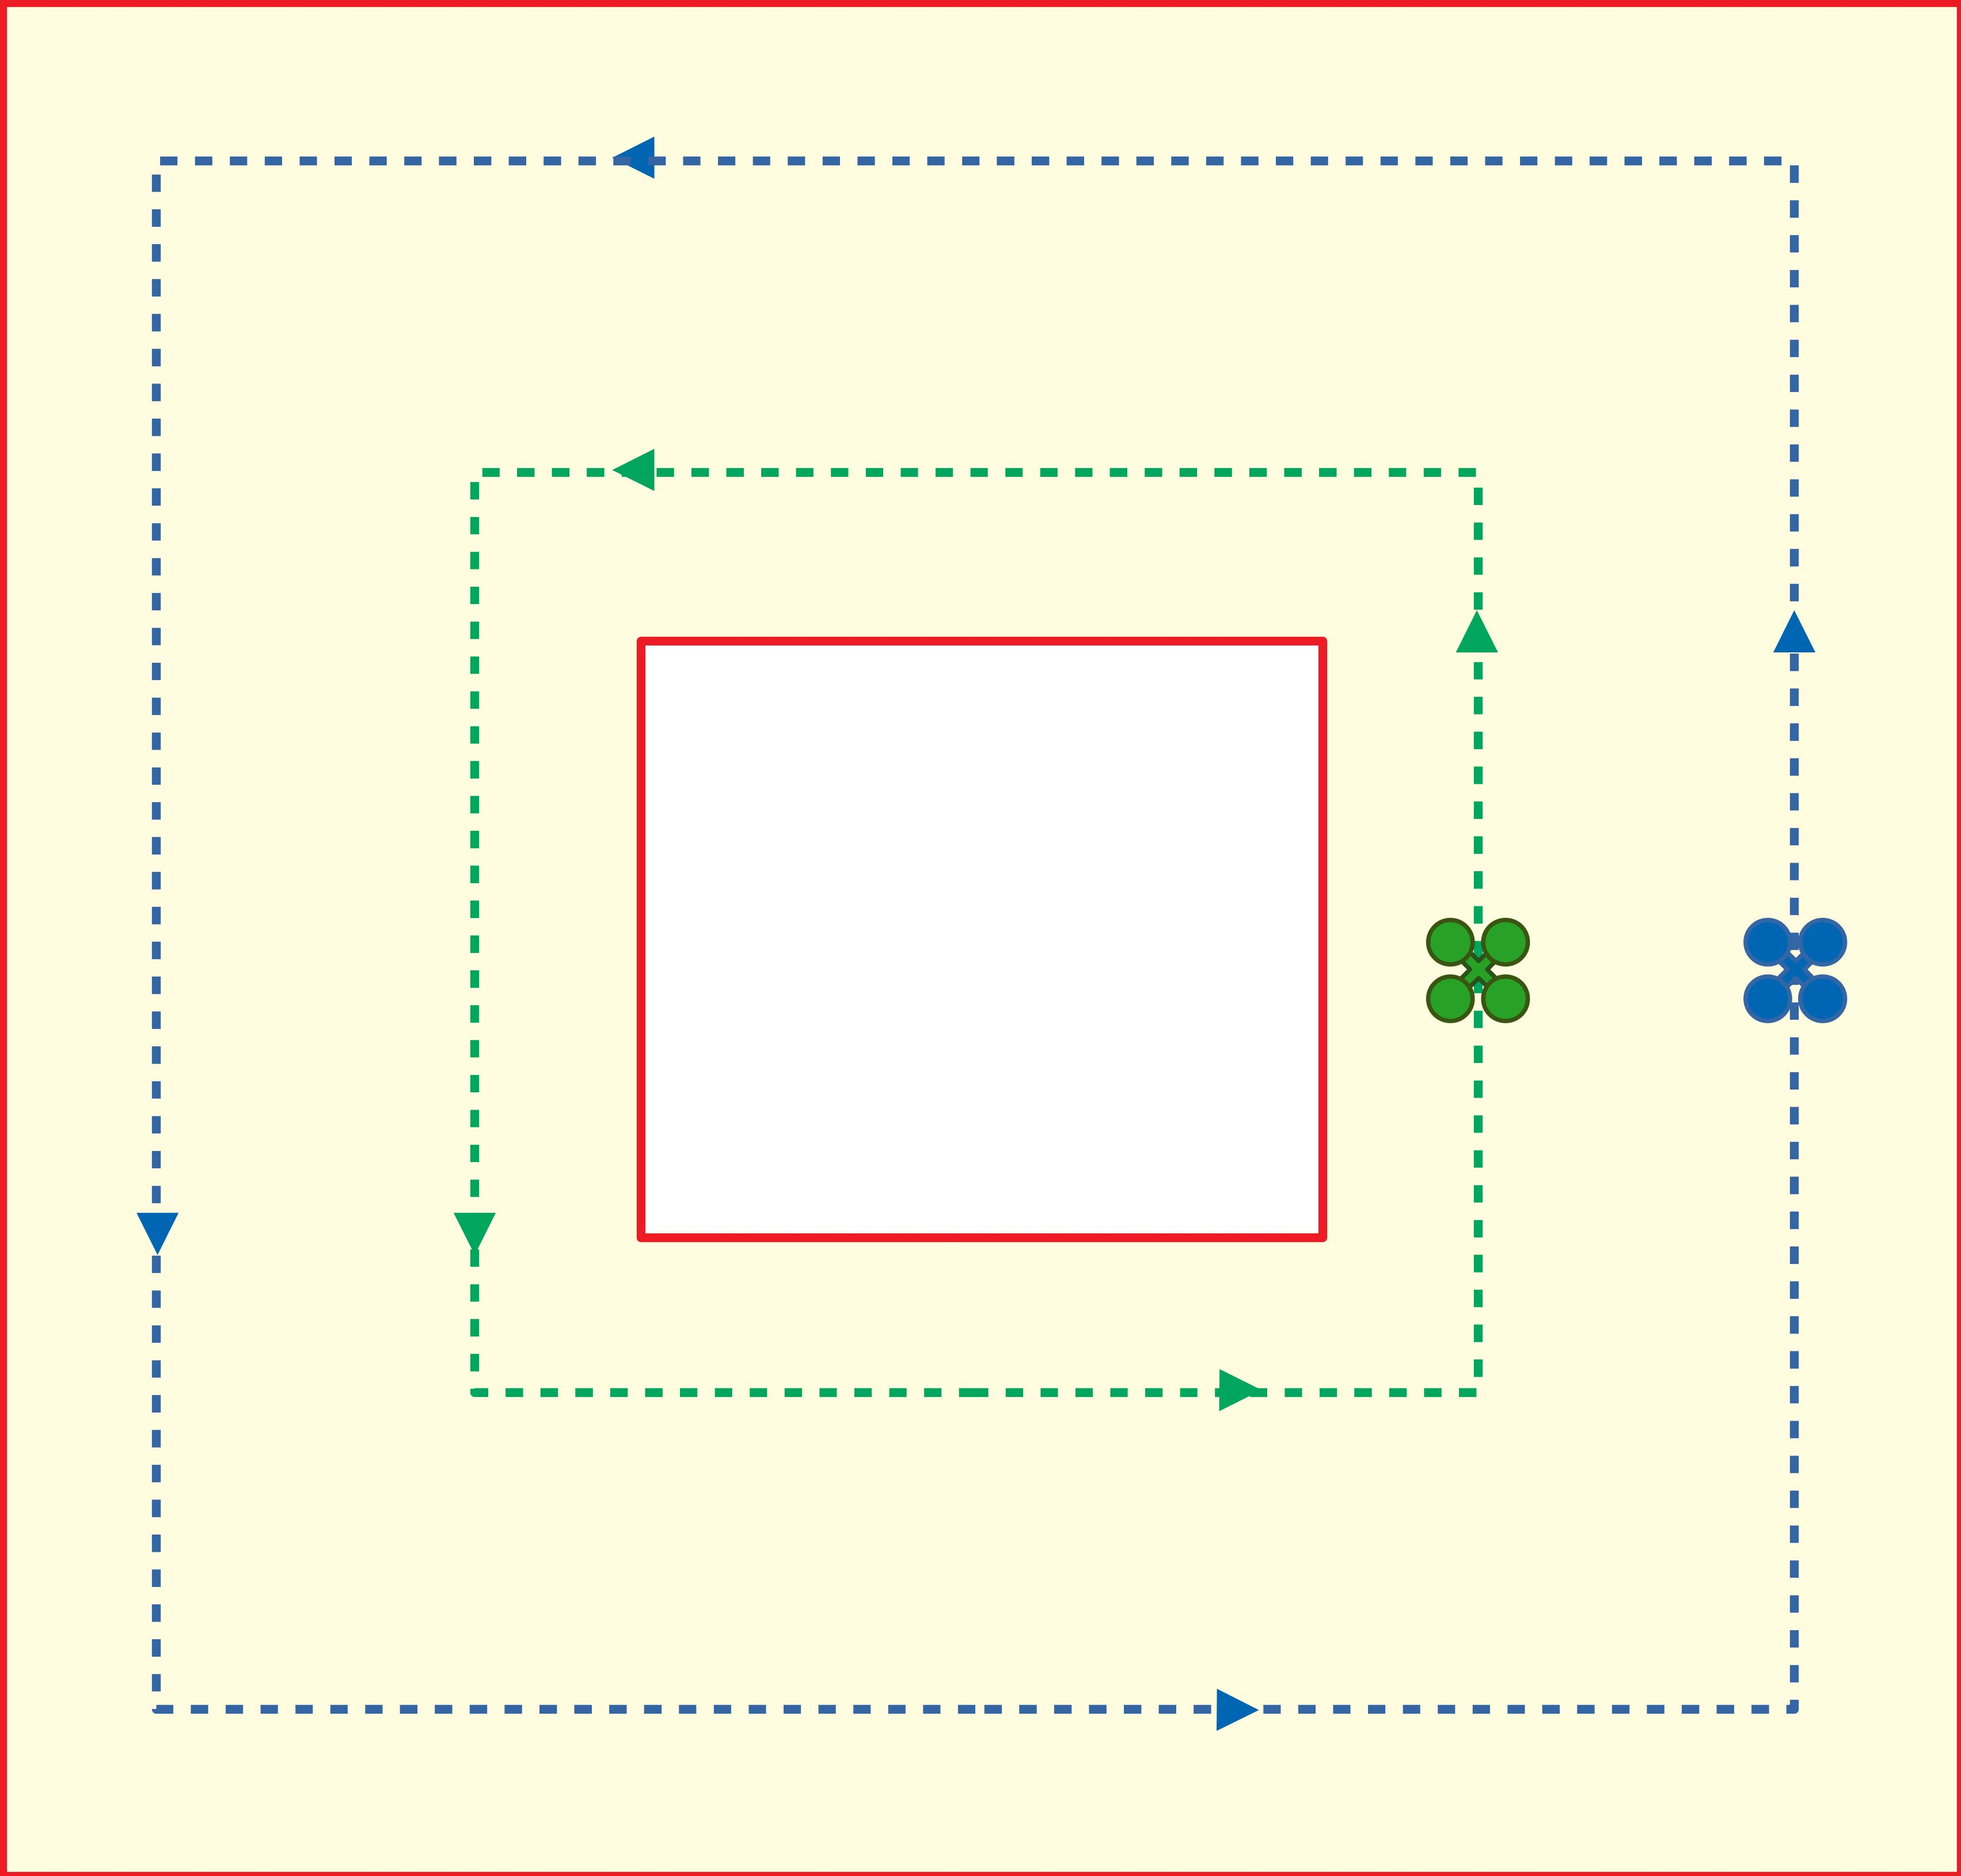
\includegraphics[scale=0.35]{assets/normal-scenario.jpg}
    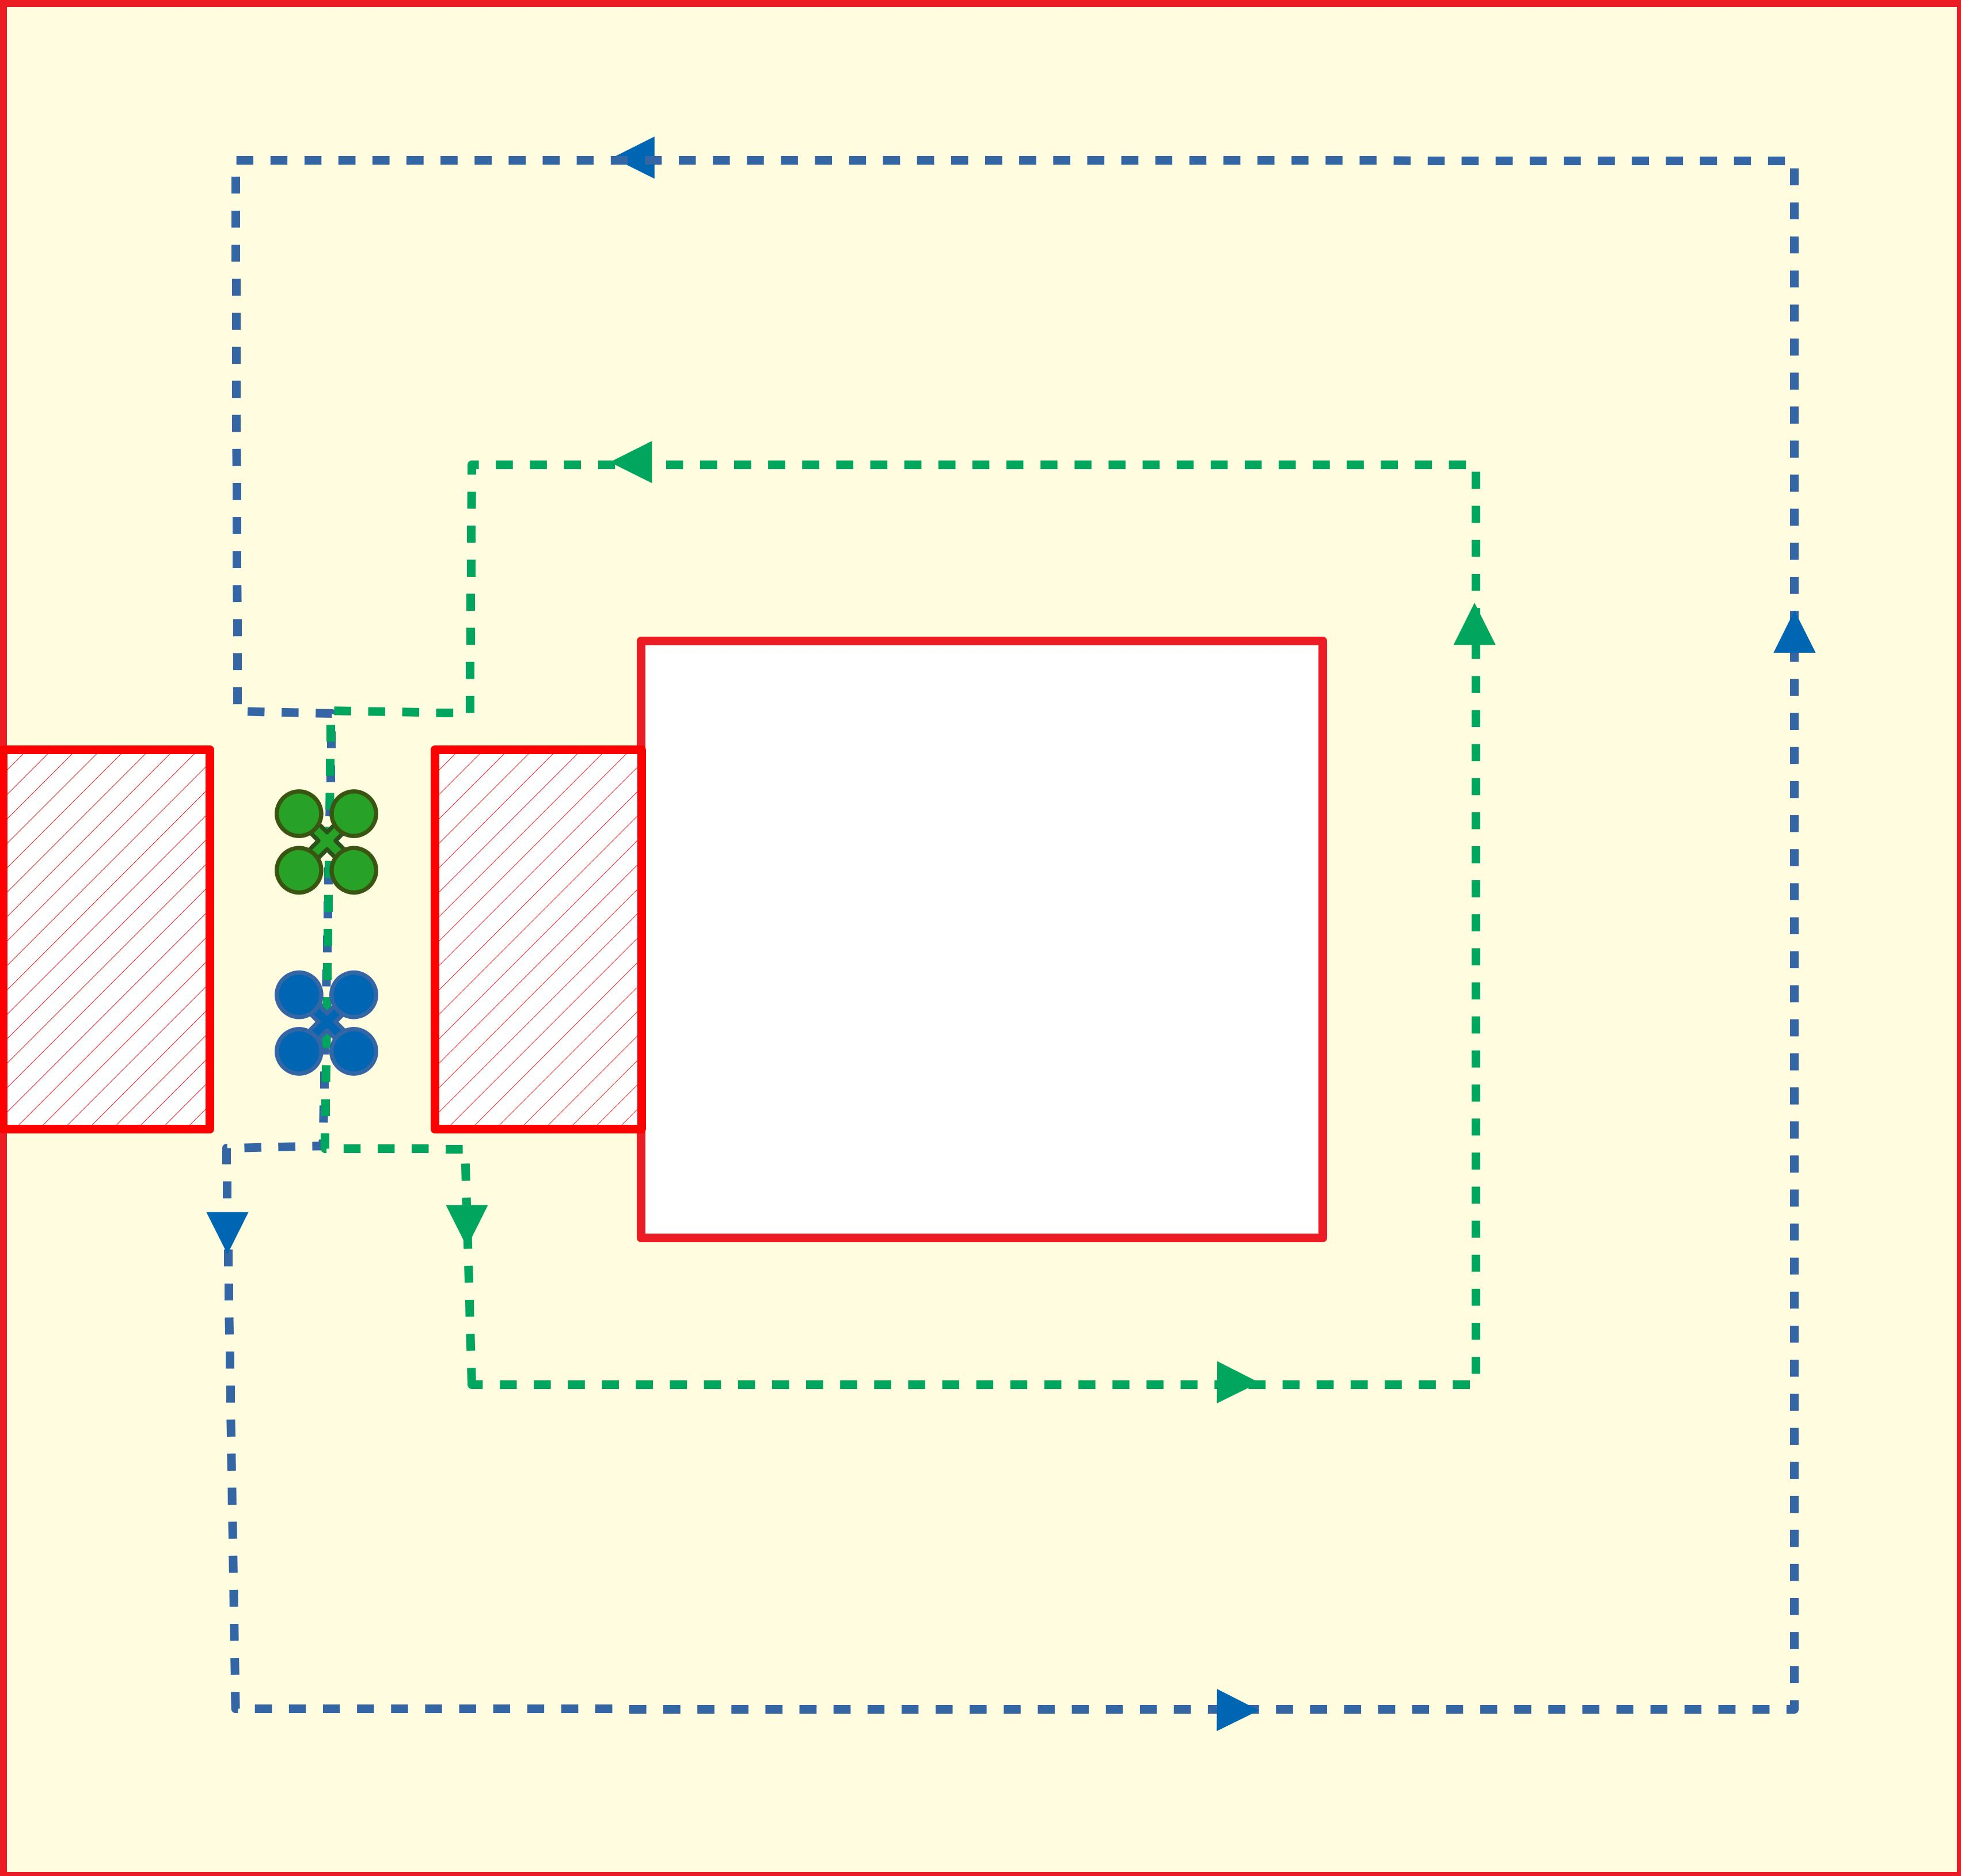
\includegraphics[scale=0.35]{assets/test-scenario.jpg}
  \caption{Two-drone leader-follower scenarios in a square (left) and a square with a blocked corridor (right). In our first set of experiments, we used the left as the reference scenario for training and the right as online testing scenario. In another experiment, we reversed training and testing scenarios.}
  \label{fig-cooperative-scenarios}
\end{figure}

\begin{figure}
  \centering
    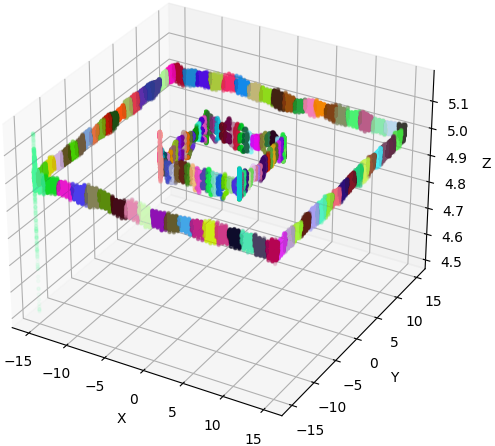
\includegraphics[scale=0.22]{assets/gps-clusters.png}
    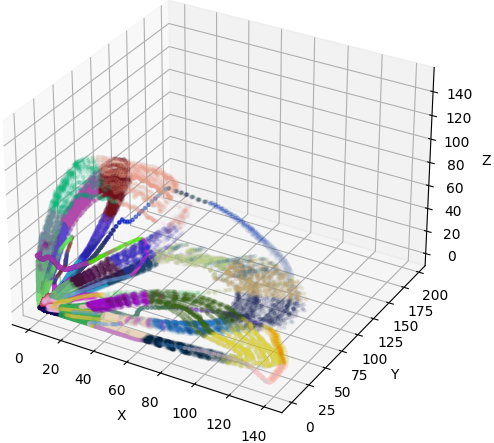
\includegraphics[scale=0.22]{assets/lidar-clusters.png}
  \caption{K-means clustering of GPS data (left) and LIDAR features (right) plotted as 3-dimensional position and feature data, respectively.}
  \label{fig-gps-lidar-clusters}
\end{figure}
For offline training, the two drones move around the square-like corridor (Figure~\ref{fig-cooperative-scenarios}, left). Figure~\ref{fig-gps-lidar-clusters} depicts the results of the K-means clustering of the GPS data (left) and the LIDAR feature data (right). We use the position and the derived velocity as input for GPS clustering which results in a nice rectangular shape in the left plot. Similarly, we use the 3-dimensional feature vector and its first derivative as input for LIDAR clustering. As shown in the right plot, moving along corridors results in a "loop" for the clustered LIDAR features. Since there is a high variation in the feature derivatives, clustering is not as robust as for GPS data (i.e., gaps among neighboring clusters and inconsistent "loops"). In our study, we use the Hausdorff distance \cite{taha-2015-an-efficient-algorithm-for-calculating-the-exact-hausdorff-distance} as an anomaly indicator to measure the distance between the observations from all involving robots and the predicted word. In all the experiments, we defined the threshold as $\mu+3\sigma$ of anomaly values from testing the normal scenario with the offline learned model.  

 \begin{figure*}[t]
      \centering
      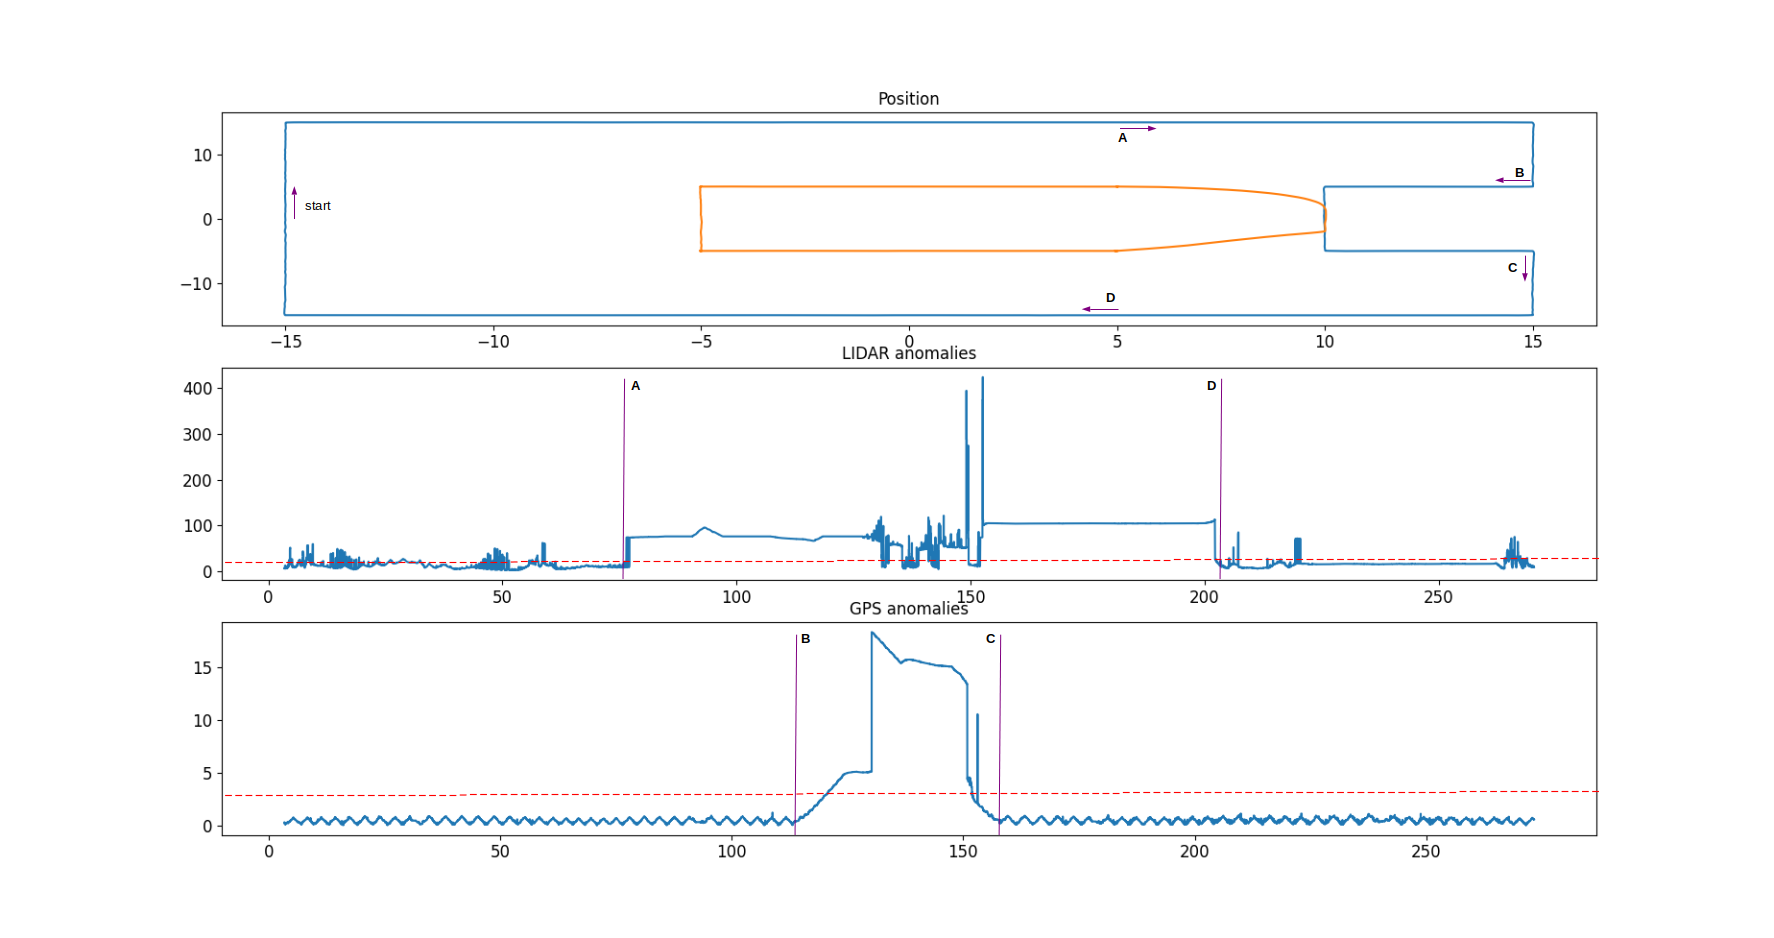
\includegraphics[width=\textwidth]{assets/anomaly-values-new-font-12.png}
      \caption{Anomaly detection in the two-drone leader-follower scenario of Figure~\ref{fig-cooperative-scenarios} right. The top graph shows the trajectories of the leader (blue) and the follower (orange) drones. The middle and bottom graphs show anomaly values for the LIDAR and GPS sensors, respectively. Purple lines indicate the time when drones move along the blocked corridor (A and D) and drones execute the obstacle avoidance maneuver (B and C). The anomaly signals derived from the sensor data significantly increase during these periods. The red dashed line is the threshold computed from $\mu+3\sigma$ of the anomaly values from testing the normal scenario with the offline learned model.}
      \label{fig-anomaly-values}
\end{figure*}

 \begin{figure*}
      \centering
      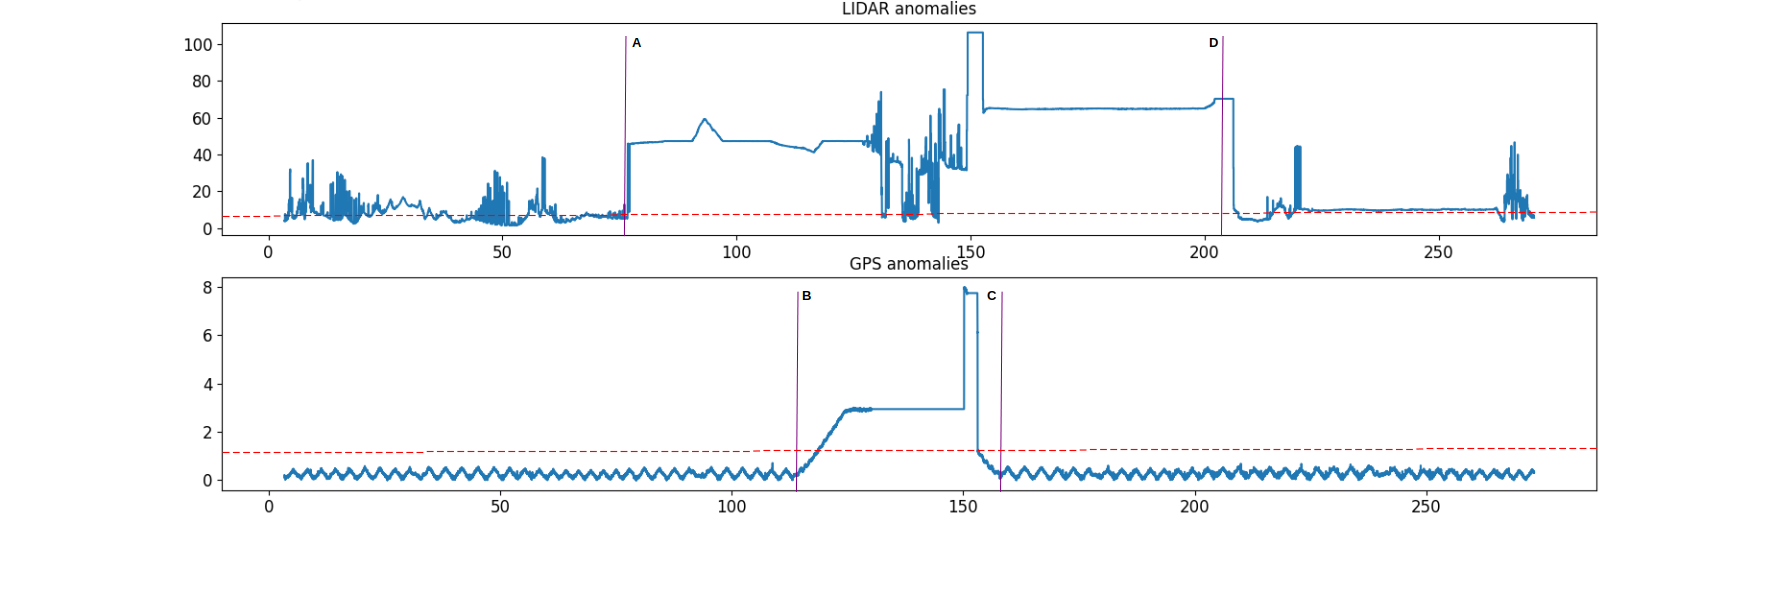
\includegraphics[width=\textwidth]{assets/aggregated-abn-vals-without-position-font-12.png}
      \caption{Anomaly detection for aggregated approach in the two-drone leader-follower scenario of Figure~\ref{fig-cooperative-scenarios} right. The anomaly signals derived from the sensor data increase less than those presented in Figure~\ref{fig-anomaly-values} during obstacle avoidance maneuver between B and C.}
      \label{fig-aggregated-anomaly-values}
\end{figure*}


   \begin{figure*}
      \centering
      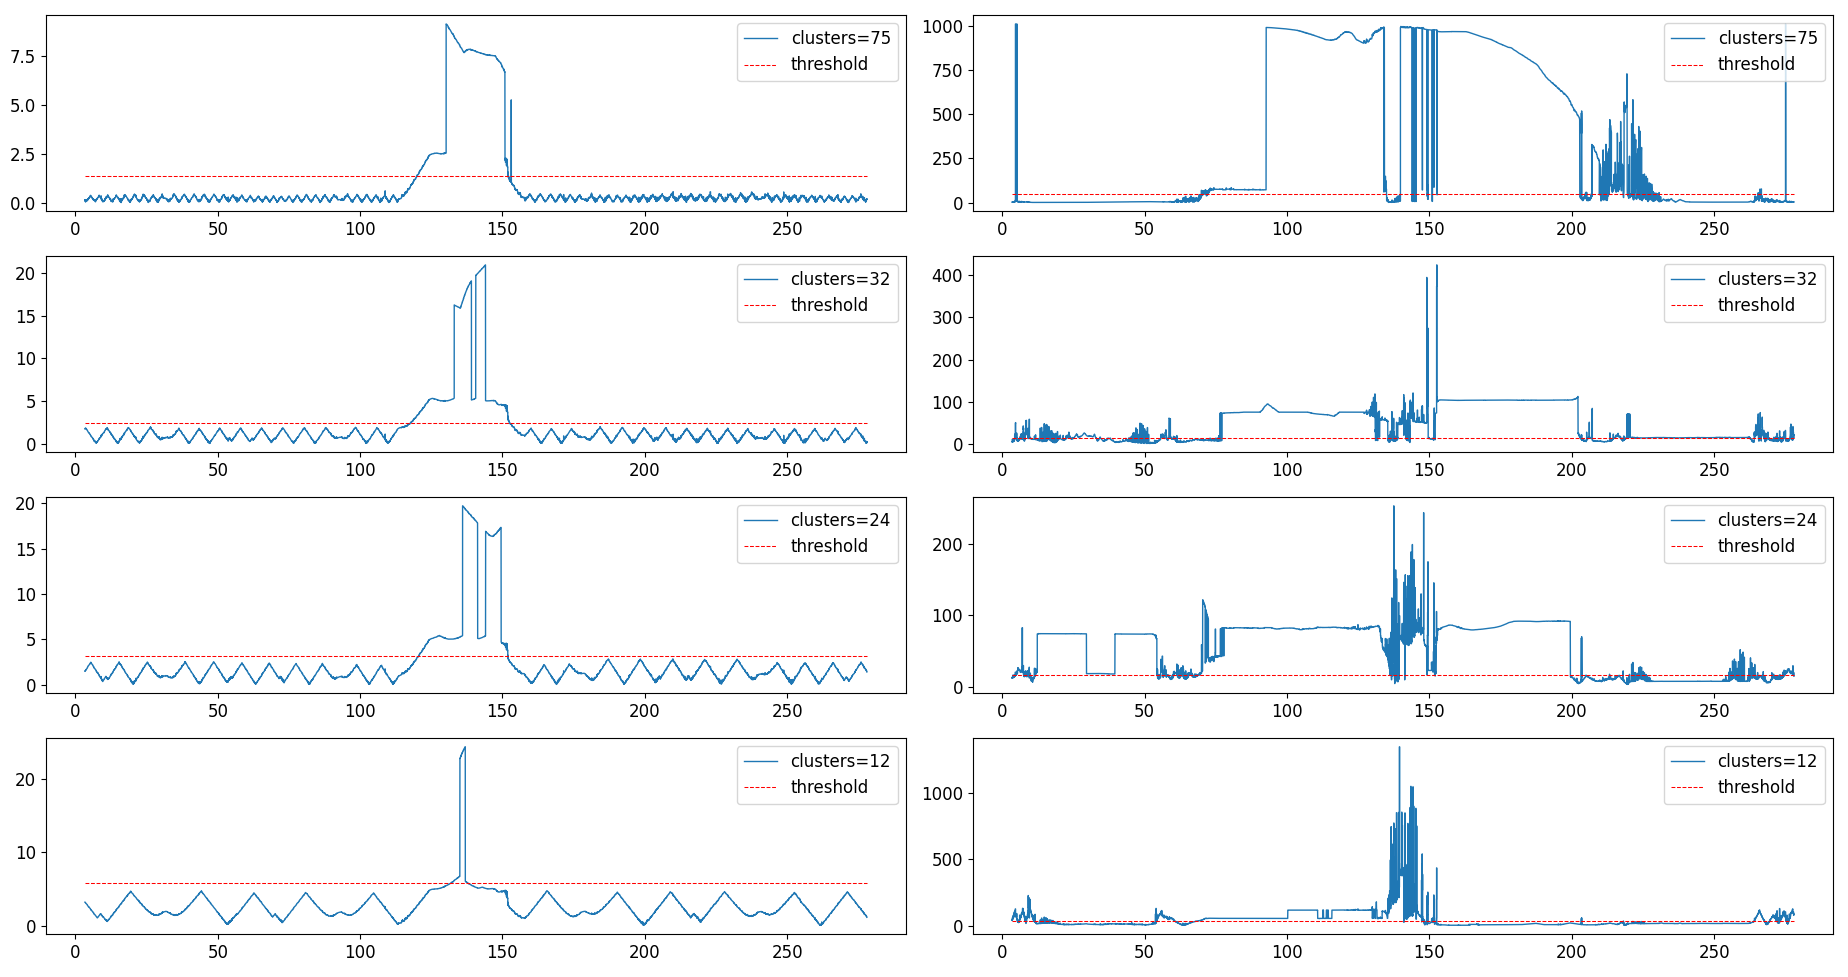
\includegraphics[width=\textwidth]{assets/gps-lidar-four-different-clusters-abn-vals.png}
      \caption{Anomaly values for GPS (left column) and LIDAR (right column) data with varying number of clusters during training (12, 24, 36 and 75 clusters from bottom to top row). With increasing number of clusters the anomaly values better reflect the deviation of the sensor data in the test scenario (GPS position during the maneuver and LIDAR reading while moving along the blocked corridor). The zigzag behavior of the GPS anomaly results from the transitions from one cluster to the next in the DBN model.
      The spikes in LIDAR anomalies are the result of the gaps between LIDAR clusters (see Figure~\ref{fig-gps-lidar-clusters} right).} 
      \label{fig-gps-lidar-four-different-clusters-abn-vals}
    \end{figure*}

Figure~\ref{fig-anomaly-values} shows the anomaly detection behavior of our approach. In this experiment, we use data from the square corridor as training data and test then the learned coupled DBNs models with data from the blocked corridor scenario. Anomalies in the drones' GPS data happen during the obstacle avoidance maneuver, which takes place between $120$ and $160$ time steps. LIDAR anomalies happen when the drones are able to "see" the obstacles with their LIDARs, basically when they move along the corridor with the obstacle, i.e., between $75$ and $200$ time steps.

We ran the experiment with the same settings for aggregated vectors to compare the results presented in Figure~\ref{fig-anomaly-values}  with the aggregated approach. The results are presented in Figure~\ref{fig-aggregated-anomaly-values}. This experiment shows that in the aggregated approach, the anomaly signals for GPS and LIDAR are $42\%$ and $38\%$ smaller than in the coupled approach. This could be interpreted as MRS's less awareness of new experiences in aggregated approach.   

In another experiment, we varied the number of clusters for the training with the two-drone leader-follower scenario (Figure~\ref{fig-cooperative-scenarios}, left), and we tested the anomaly detection with the blocked scenario (Figure~\ref{fig-cooperative-scenarios}, right). Figure~\ref{fig-gps-lidar-four-different-clusters-abn-vals} shows the results of this experiment. As the number of clusters increases, high anomaly values are better detectable in the expected regions (regions with deviations in training and test scenarios).    
Figure~\ref{fig-gps-lidar-four-different-noises-abn-vals} depicts the results of a similar experiment with a fixed number of clusters but varying noise levels.
     \begin{figure*}
      \centering
      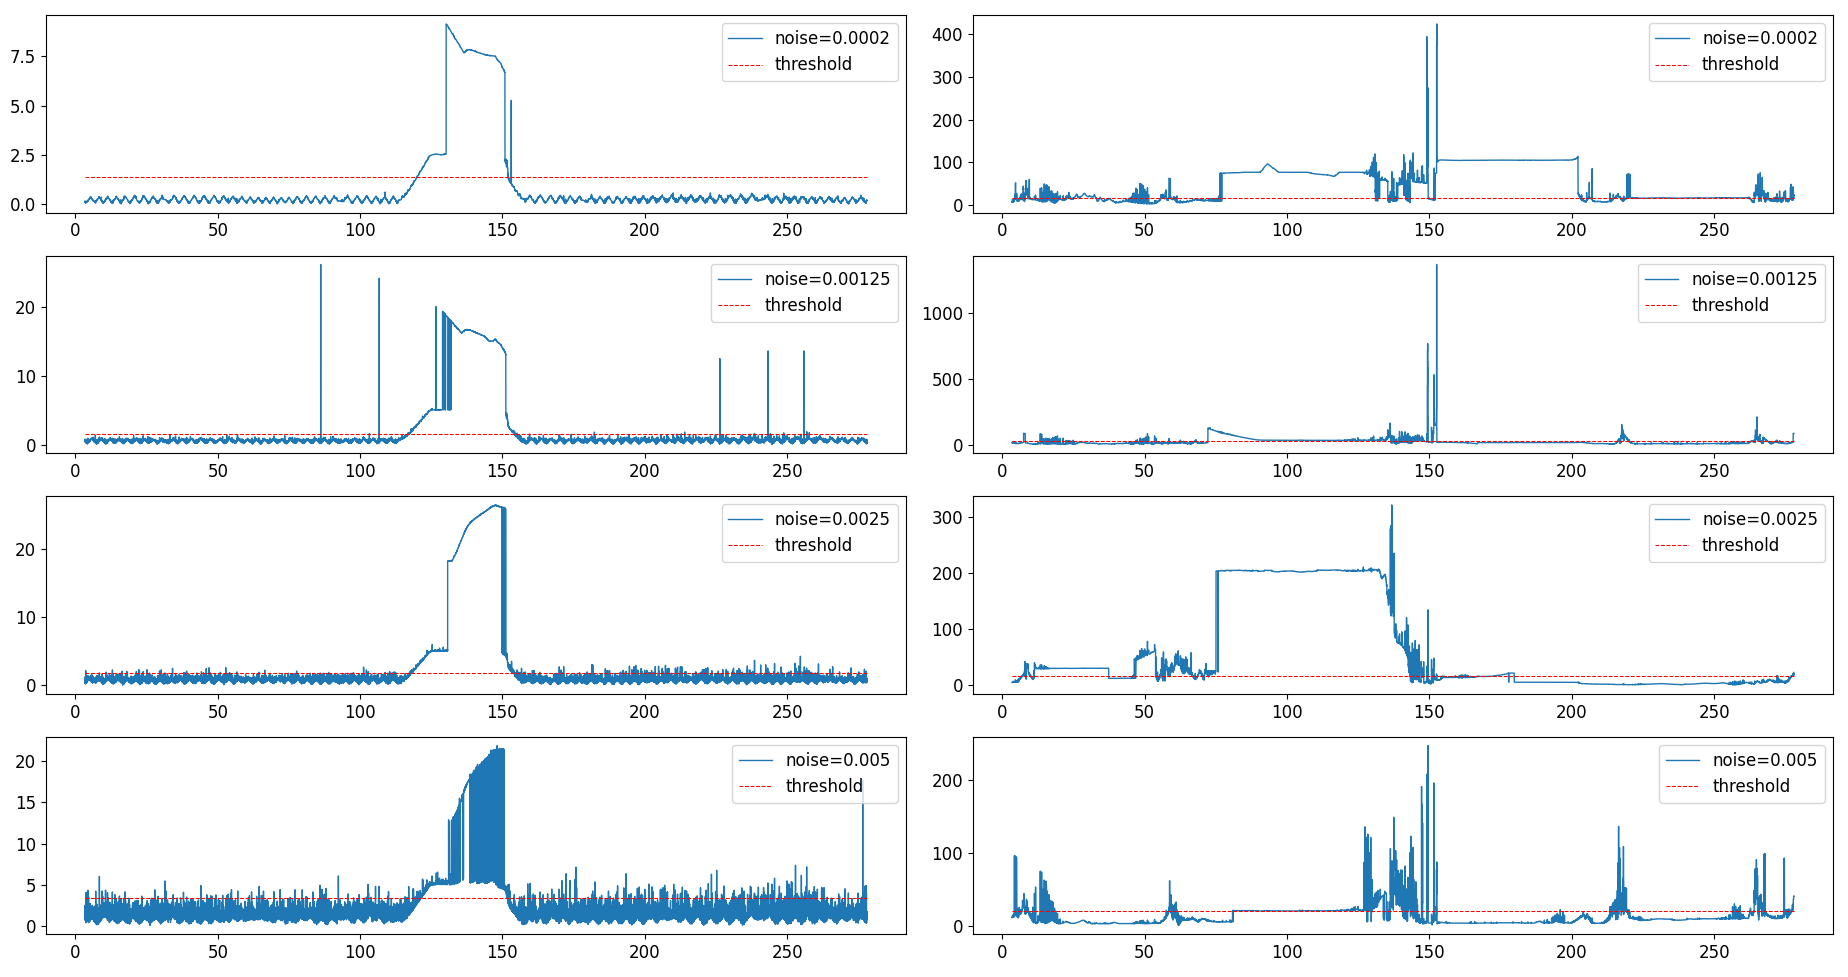
\includegraphics[width=\textwidth]{assets/gps-lidar-four-different-noises-abn-vals.png}
      \caption{Anomaly values for GPS (left column) and LIDAR (right column) data with varying sensor noise level (20, 125, 200 and 500 $\cdot 10^{-5}$ from top to bottom row) for training and test. The spikes in LIDAR anomalies are the result of the gaps between LIDAR clusters (see Figure~\ref{fig-gps-lidar-clusters} right). Comparing lowest left and right graphs, it is visible that the autoencoder was successful in significantly reducing the spikes for LIDAR data.}
      \label{fig-gps-lidar-four-different-noises-abn-vals}
    \end{figure*}

\section{Conclusion}
\label{sec-conclusion}
We introduced a causal-temporal model based on coupled hierarchical dynamic Bayesian networks for anomaly detection in multi-robot systems. As demonstrated in our simulation study, this approach results in high anomaly values for regions where the robots' behaviors deviate between training and testing. Proprioceptive and exteroceptive hierarchical models help to abstract the robots' behavior and trigger building new models. Our approach is a work in progress and currently faces limitations regarding the accuracy of LIDAR anomaly data, the robustness to noise in the sensor data, and the scaling to multi-robot systems with a larger number of robots. In future work, we plan to address the aforementioned limitations and to extend our approach towards model generation and model selection---two key capabilities of self-aware autonomous systems.
\bibliographystyle{IEEEtran}
\bibliography{refs}
\end{document}
